\documentclass[a4paper,twocolumn]{article}
\usepackage[UTF8]{ctex}
\usepackage{setspace}
\usepackage{amsmath, amsthm}
\usepackage{listings,xcolor}
\usepackage{geometry} % 设置页边距
\usepackage{fontspec}
\usepackage{graphicx}
\usepackage{fancyhdr} % 自定义页眉页脚
\setsansfont{Consolas} % 设置英文字体
\setmonofont[Mapping={}]{Consolas} % 英文引号之类的正常显示,相当于设置英文字体
\geometry{left=1cm,right=1cm,top=2cm,bottom=0.5cm} % 页边距
\setlength{\columnsep}{30pt}
% \setlength\columnseprule{0.4pt} % 分割线
%==============================常用宏包、环境==============================%

%==============================页眉、页脚、代码格式设置==============================%
% 页眉、页脚设置
\pagestyle{fancy}
% \lhead{CUMTB}
\lhead{\CJKfamily{hei} ACM-ICPC Template by tokitsukaze}
\chead{}
% \rhead{Page \thepage}
\rhead{\CJKfamily{hei} 第 \thepage 页}
\lfoot{}
\cfoot{}
\rfoot{}
\renewcommand{\headrulewidth}{0.4pt}
\renewcommand{\footrulewidth}{0.4pt}




\lstset{
    language    = c++,
    numbers     = left,
    numberstyle = \tiny,
    breaklines  = true,
    captionpos  = b,
    tabsize     = 4,
    frame       = single,
    columns     = fullflexible,
    commentstyle = \color[RGB]{0,128,0},
    keywordstyle = \color[RGB]{0,0,255},
    basicstyle   = \small\ttfamily,
    stringstyle  = \color[RGB]{148,0,209}\ttfamily,
    rulesepcolor = \color{red!20!green!20!blue!20},
    showstringspaces = false,
}


\title{ACM-ICPC Template}
\author {tokitsukaze}

\begin{document}
\begin{titlepage}
\maketitle
\vspace*{50pt}
\begin{center}


\includegraphics[width=4in]{1.png}
\end{center}
\end{titlepage}
\newpage
\pagestyle{empty}
\renewcommand{\contentsname}{目录}
\tableofcontents
\newpage\clearpage
\newpage
\pagestyle{fancy}
\setcounter{page}{1}

\section{字符串}
\subsection{KMP}
\subsubsection{KMP}
\lstinputlisting{字符串/KMP/KMP.cpp}
\subsubsection{exKMP}
\lstinputlisting{字符串/KMP/exKMP.cpp}
\subsection{Hash}
\subsubsection{hash}
\lstinputlisting{字符串/Hash/hash.cpp}
\subsubsection{hash\_map}
\lstinputlisting{字符串/Hash/hash_map.cpp}
\subsubsection{BKDRHash}
\lstinputlisting{字符串/Hash/BKDRHash.cpp}
\subsection{Manacher}
\subsubsection{插字符}
\lstinputlisting{字符串/Manacher/Manacher-插字符.cpp}
\subsubsection{不插字符}
\lstinputlisting{字符串/Manacher/Manacher-不插字符.cpp}
\subsection{后缀数组}
\subsubsection{倍增sa}
\lstinputlisting{字符串/后缀数组/倍增sa.cpp}
\subsubsection{SA-IS}
\lstinputlisting{字符串/后缀数组/sais.cpp}
\subsection{自动机}
\subsubsection{AC自动机}
\lstinputlisting{字符串/自动机/AC自动机.cpp}
\subsubsection{大字符集AC自动机}
\lstinputlisting{字符串/自动机/大字符集AC自动机.cpp}
\subsubsection{后缀自动机}
\lstinputlisting{字符串/自动机/后缀自动机.cpp}
\subsubsection{回文自动机}
\lstinputlisting{字符串/自动机/回文自动机.cpp}
\subsubsection{序列自动机}
\lstinputlisting{字符串/自动机/序列自动机.cpp}
\subsection{最小表示法}
\subsubsection{最小表示法}
\lstinputlisting{字符串/最小表示法/最小表示法.cpp}
\subsubsection{最大表示法}
\lstinputlisting{字符串/最小表示法/最大表示法.cpp}
\subsection{shift\_and}
\lstinputlisting{字符串/shift_and.cpp}
\section{数据结构}
\subsection{RMQ}
\subsubsection{一维RMQ}
\lstinputlisting{数据结构/RMQ/一维RMQ.cpp}
\subsubsection{二维RMQ}
\lstinputlisting{数据结构/RMQ/二维RMQ.cpp}
\subsection{单调队列}
\lstinputlisting{数据结构/单调队列.cpp}
\subsection{LCA}
\subsubsection{倍增LCA}
\lstinputlisting{数据结构/LCA/倍增LCA.cpp}
\subsubsection{RMQ维护欧拉序求LCA}
\lstinputlisting{数据结构/LCA/RMQ维护欧拉序求LCA.cpp}
\subsection{轻重链剖分}
\begin{spacing}{1.5}
-----------------------------------------------------------------------\\
size[]数组,以x为根的子树节点个数。\\
top[]数组,当前节点的所在链的顶端节点。\\
son[]数组,重儿子。\\
deep[]数组,当前节点的深度。\\
fa[]数组,当前节点的父亲。\\
idx[]数组,树中每个节点剖分后的新编号。\\
rnk[]数组,idx的逆,表示线段上中当前位置表示哪个节点。 

\end{spacing}
\lstinputlisting{数据结构/轻重链剖分.cpp}
\subsection{并查集}
\subsubsection{并查集}
\lstinputlisting{数据结构/并查集/并查集.cpp}
\subsubsection{map实现并查集}
\lstinputlisting{数据结构/并查集/map实现并查集.cpp}
\subsubsection{可撤销并查集}
\lstinputlisting{数据结构/并查集/可撤销并查集.cpp}
\subsection{树状数组}
\subsubsection{一维单点BIT}
\lstinputlisting{数据结构/树状数组/一维单点BIT.cpp}
\subsubsection{一维区间BIT}
\lstinputlisting{数据结构/树状数组/一维区间BIT.cpp}
\subsubsection{二维单点BIT}
\lstinputlisting{数据结构/树状数组/二维单点BIT.cpp}
\subsection{线段树}
\subsubsection{线段树}
\lstinputlisting{数据结构/线段树/线段树.cpp}
\subsubsection{动态开点线段树}
\lstinputlisting{数据结构/线段树/动态开点线段树.cpp}
\subsubsection{线段树套线段树}
\lstinputlisting{数据结构/线段树/线段树套线段树.cpp}
\subsubsection{线段树分裂合并}
\lstinputlisting{数据结构/线段树/线段树分裂合并.cpp}
\subsection{主席树}
\lstinputlisting{数据结构/主席树.cpp}
\subsection{李超树}
\lstinputlisting{数据结构/李超树.cpp}
\subsection{平衡树}
\subsubsection{Treap}
\lstinputlisting{数据结构/平衡树/Treap.cpp}
\subsection{字典树}
\subsubsection{trie}
\lstinputlisting{数据结构/字典树/trie.cpp}
\subsubsection{01trie}
\lstinputlisting{数据结构/字典树/01trie.cpp}
\subsection{kd-tree}
\lstinputlisting{数据结构/kd-tree.cpp}
\subsection{虚树}
\lstinputlisting{数据结构/虚树.cpp}
\subsection{pbds可并堆}
\lstinputlisting{数据结构/pbds可并堆.cpp}
\subsection{k叉哈夫曼树}
\begin{spacing}{1.5}
-----------------------------------------------------------------------\\
用两个队列代替优先队列 复杂度O(n)\\
注意:小的先进 原数组有序

\end{spacing}
\lstinputlisting{数据结构/k叉哈夫曼树.cpp}
\subsection{笛卡尔树}
\begin{spacing}{1.5}
-----------------------------------------------------------------------\\
O(n)构造笛卡尔树 返回根\\
性质:\\
1.树中的元素满足二叉搜索树性质,要求按照中序遍历得到的序列为原数组序列\\
2.树中节点满足堆性质,节点的key值要大于其左右子节点的key值

\end{spacing}
\lstinputlisting{数据结构/笛卡尔树.cpp}
\subsection{析合树}
\begin{spacing}{1.5}
-----------------------------------------------------------------------\\
id[x]:序列中第x个数在析合树上的编号。\\
l[x],r[x]:节点x的作用域。\\
type[x]:节点x的类型,0表示析点,1表示合点,默认叶子节点为析点。\\
注意:若一个节点为合点,这个节点的儿子序列有序。
析合树举例:\\
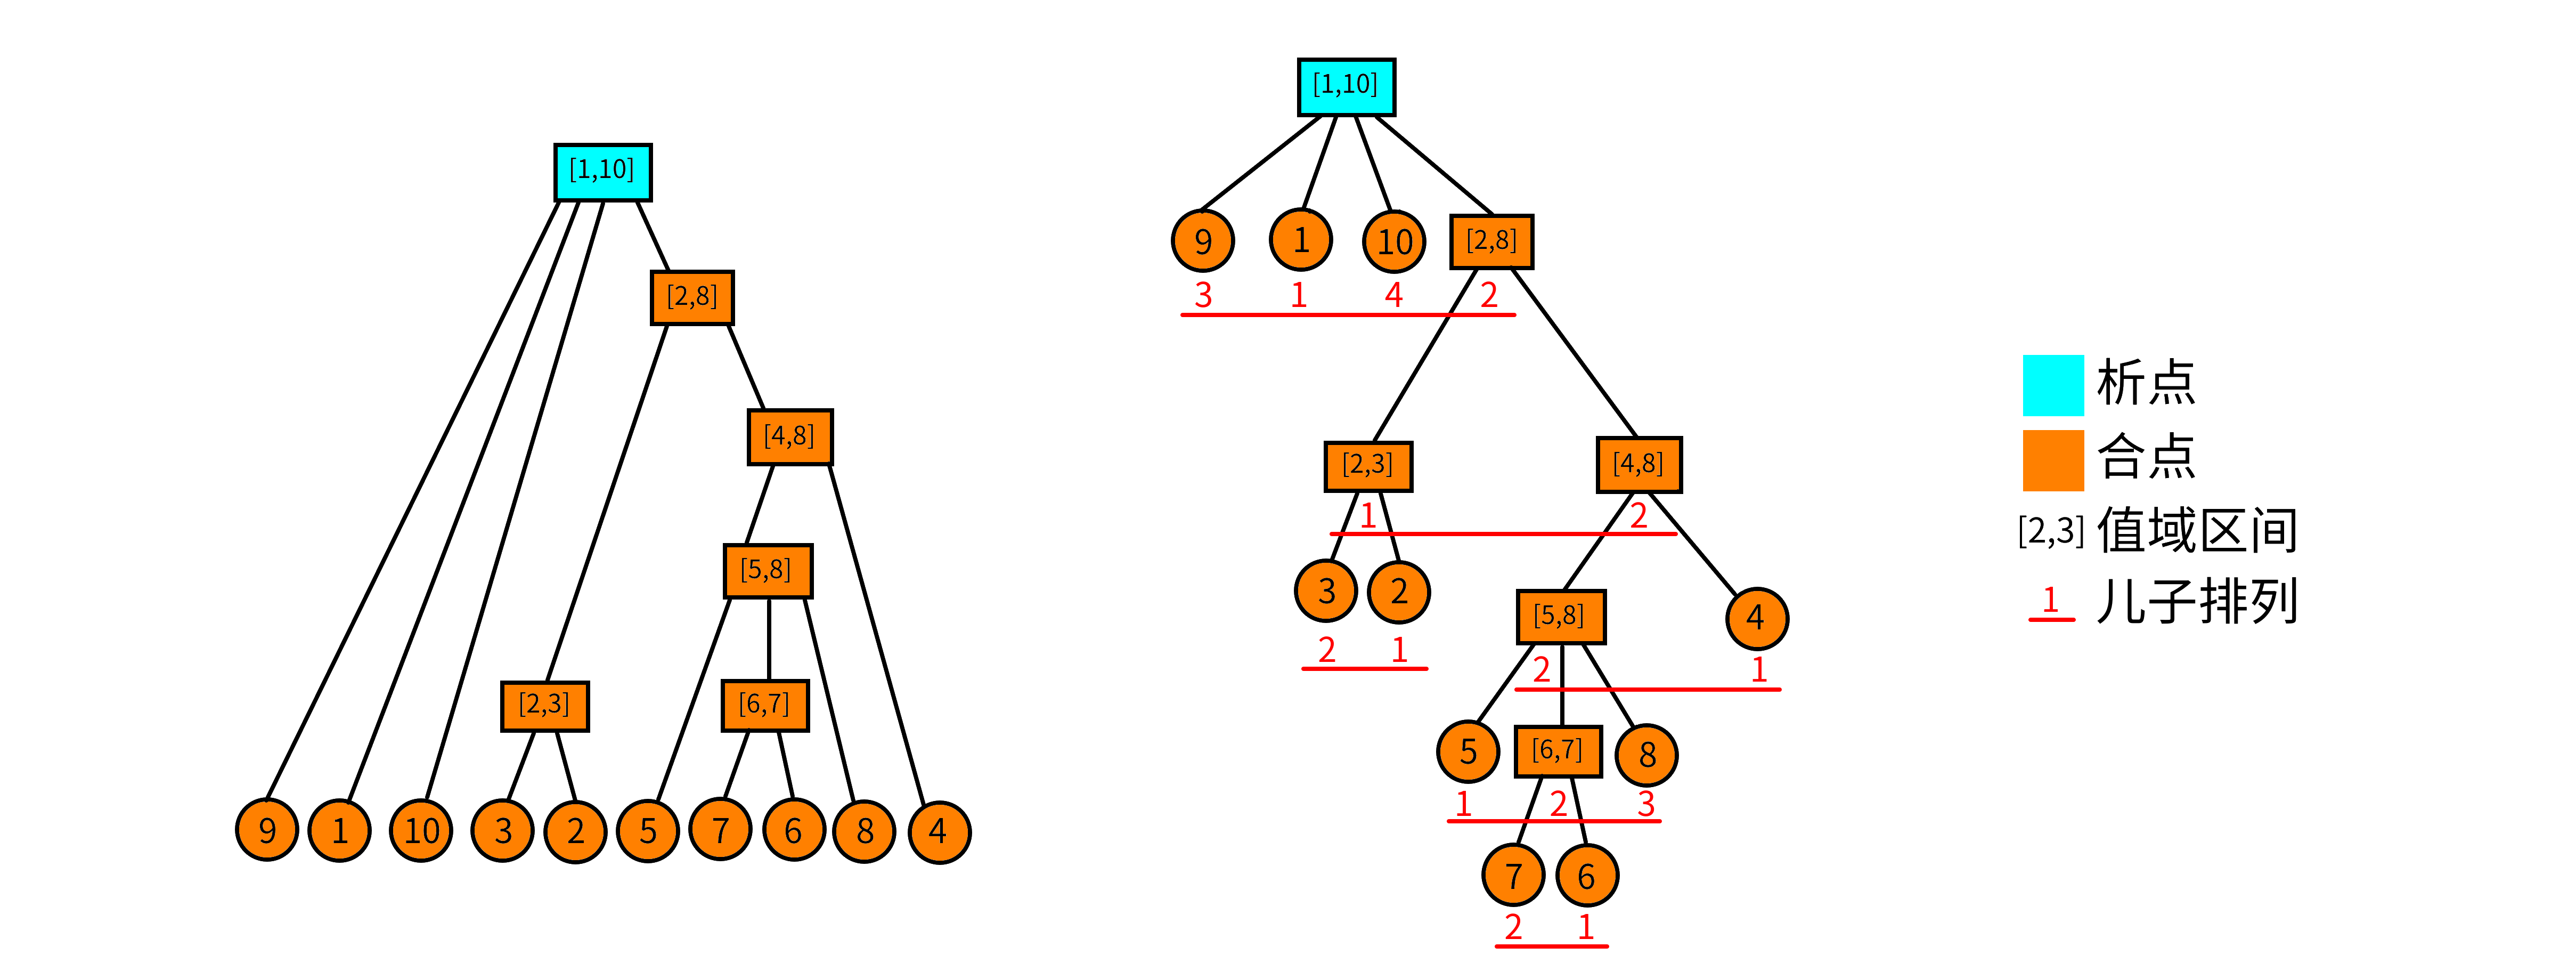
\includegraphics[width=4in]{div-com1.png}

\end{spacing}
\lstinputlisting{数据结构/析合树.cpp}
\section{图论}
\subsection{链式前向星}
\lstinputlisting{图论/链式前向星.cpp}
\subsection{最短路}
\subsubsection{dijkstra}
\lstinputlisting{图论/最短路/dijkstra.cpp}
\subsubsection{spfa}
\lstinputlisting{图论/最短路/spfa.cpp}
\subsubsection{floyd求最小环}
\lstinputlisting{图论/最短路/floyd求最小环.cpp}
\subsection{最小生成树}
\subsubsection{kruskal}
\lstinputlisting{图论/最小生成树/kruskal.cpp}
\subsubsection{prim}
\lstinputlisting{图论/最小生成树/prim.cpp}
\subsection{二分图匹配}
\subsubsection{匈牙利算法}
\lstinputlisting{图论/二分图匹配/匈牙利算法.cpp}
\subsubsection{二分图带权匹配}
\lstinputlisting{图论/二分图匹配/二分图带权匹配.cpp}
\subsection{最大流}
\subsubsection{dinic}
\lstinputlisting{图论/最大流/dinic.cpp}
\subsubsection{ISAP}
\lstinputlisting{图论/最大流/ISAP.cpp}
\subsubsection{high-level-preflow-push}
\lstinputlisting{图论/最大流/high-level-preflow-push.cpp}
\subsection{最小费用最大流}
\subsubsection{spfa费用流}
\lstinputlisting{图论/最小费用最大流/spfa费用流.cpp}
\subsubsection{dijkstra费用流}
\lstinputlisting{图论/最小费用最大流/dijkstra费用流.cpp}
\subsection{强连通分量}
\lstinputlisting{图论/强连通分量.cpp}
\subsection{双联通分量}
\subsubsection{边双连通}
\lstinputlisting{图论/双联通分量/边双连通.cpp}
\subsection{团}
\subsubsection{最大团}
\lstinputlisting{图论/团/最大团.cpp}
\subsubsection{极大团计数}
\lstinputlisting{图论/团/极大团计数.cpp}
\subsection{拓扑排序}
\lstinputlisting{图论/拓扑排序.cpp}
\subsection{2-sat}
\subsubsection{2-sat输出任意解}
\lstinputlisting{图论/2-sat/2-sat输出任意解.cpp}
\subsubsection{2-sat字典序最小解}
\lstinputlisting{图论/2-sat/2-sat字典序最小解.cpp}
\subsection{支配树}
\lstinputlisting{图论/支配树.cpp}
\section{数论}
\subsection{素数筛}
\subsubsection{埃筛}
\lstinputlisting{数论/素数筛/埃筛.cpp}
\subsubsection{线性筛}
\lstinputlisting{数论/素数筛/线性筛.cpp}
\subsubsection{区间筛}
\lstinputlisting{数论/素数筛/区间筛.cpp}
\subsection{扩展欧几里得}
\subsubsection{exgcd}
\lstinputlisting{数论/扩展欧几里得/exgcd.cpp}
\subsubsection{ax+by=c}
\lstinputlisting{数论/扩展欧几里得/ax+by=c.cpp}
\subsubsection{exgcd求逆元}
\lstinputlisting{数论/扩展欧几里得/exgcd求逆元.cpp}
\subsection{中国剩余定理}
\subsubsection{CRT}
\lstinputlisting{数论/中国剩余定理/CRT.cpp}
\subsubsection{exCRT}
\lstinputlisting{数论/中国剩余定理/exCRT.cpp}
\subsection{组合数}
\subsubsection{打表}
\lstinputlisting{数论/组合数/打表.cpp}
\subsubsection{预处理}
\lstinputlisting{数论/组合数/预处理.cpp}
\subsubsection{Lucas定理}
\lstinputlisting{数论/组合数/Lucas定理.cpp}
\subsubsection{exLucas}
\lstinputlisting{数论/组合数/exLucas.cpp}
\subsection{欧拉函数}
\begin{spacing}{1.5}
<=n且与n互质的数的和:n*phi[n]/2
\end{spacing}
\subsubsection{直接求}
\lstinputlisting{数论/欧拉函数/直接求.cpp}
\subsubsection{线性筛}
\lstinputlisting{数论/欧拉函数/线性筛.cpp}
\subsection{莫比乌斯函数}
\lstinputlisting{数论/莫比乌斯函数.cpp}
\subsection{Berlekamp-Massey}
\lstinputlisting{数论/Berlekamp-Massey.cpp}
\subsection{exBSGS}
\lstinputlisting{数论/exBSGS.cpp}
\subsection{Miller\_Rabin+Pollard\_rho}
\lstinputlisting{数论/Miller_Rabin+Pollard_rho.cpp}
\subsection{第二类Stirling数}
\lstinputlisting{数论/第二类Stirling数.cpp}
\subsection{原根}
\begin{spacing}{1.5}
-----------------------------------------------------------------------\\
原根性质\\
1.一个数m如果有原根,则其原根个数为$phi[phi[m]]$。若m为素数,则其原根个数为$phi[phi[m]]=phi[m-1]$。\\
2.有原根的数只有$2,4,p^n,2*p^n$ (p为质数,n为正整数)\\
3.一个数的最小原根的大小是$O(n^{0.25})$的\\
4.如果g为n的原根,则$g^d$为n的原根的充要条件是$gcd(d,phi[n])=1$\\
\\
指标法则\\
1. $I(a*b)≡I(a)+I(b) (mod p-1)$\\
2. $I(a^k)≡k*I(a) (mod p-1)$

\end{spacing}
\lstinputlisting{数论/原根.cpp}
\subsection{二次剩余}
\lstinputlisting{数论/二次剩余.cpp}
\section{多项式}
\subsection{FFT}
\lstinputlisting{多项式/FFT.cpp}
\subsection{NTT}
\lstinputlisting{多项式/NTT.cpp}
\subsection{FWT}
\lstinputlisting{多项式/FWT.cpp}
\subsection{拉格朗日插值}
\lstinputlisting{多项式/拉格朗日插值.cpp}
\section{矩阵}
\subsection{矩阵类}
\lstinputlisting{矩阵/矩阵类.cpp}
\subsection{高斯消元}
\subsubsection{同余方程}
\lstinputlisting{矩阵/高斯消元/同余方程.cpp}
\subsubsection{同余方程mod=2}
\lstinputlisting{矩阵/高斯消元/同余方程mod=2.cpp}
\subsection{单纯形}
\lstinputlisting{矩阵/单纯形.cpp}
\subsection{线性基}
\lstinputlisting{矩阵/线性基.cpp}
\section{博弈}
\subsection{SG函数}
\begin{spacing}{1.5}
-----------------------------------------------------------------------\\
f[m]:可改变当前状态的方式,N为方式的种类,要先从小到大sort\\
sg[]:sg表\\
flag[m]:为x后继状态的集合

\end{spacing}
\subsubsection{sg表}
\lstinputlisting{博弈/SG函数/sg表.cpp}
\subsubsection{记忆化搜索求sg函数}
\lstinputlisting{博弈/SG函数/记忆化搜索求sg函数.cpp}
\subsection{结论}
\begin{spacing}{1.5}
-----------------------------------------------------------------------\\
1.阶梯博弈\\
0层为终点的阶梯博弈,等价于奇数层的nim,偶数层的移动不影响结果 \\
\\
2.SJ定理\\
对于任意一个Anti-SG游戏,如果我们规定当局面中所有的单一游戏的SG值为0时,游戏结束。\\
先手必胜当且仅当:\\
(1)游戏的SG函数不为0且游戏中某个单一游戏的SG函数大于1;\\
(2)游戏的SG函数为0且游戏中没有单一游戏的SG函数大于1。
\end{spacing}
\section{dp}
\subsection{LIS}
\lstinputlisting{dp/LIS.cpp}
\subsection{LPS}
\lstinputlisting{dp/LPS.cpp}
\subsection{数位dp}
\lstinputlisting{dp/数位dp.cpp}
\section{杂项}
\subsection{FastIO}
\lstinputlisting{杂项/FastIO.cpp}
\subsection{O(1)快速乘}
\lstinputlisting{杂项/快速乘.cpp}
\subsection{快速模}
\lstinputlisting{杂项/快速模.cpp}
\subsection{xor\_sum(1,n)}
\lstinputlisting{杂项/xor_sum.cpp}
\subsection{约瑟夫环kth}
\lstinputlisting{杂项/约瑟夫环kth.cpp}
\subsection{判断星期几}
\lstinputlisting{杂项/判断星期几.cpp}
\subsection{离散化}
\lstinputlisting{杂项/离散化.cpp}
\subsection{网格整数点正方形个数}
\lstinputlisting{杂项/网格整数点正方形个数.cpp}
\subsection{模拟退火}
\lstinputlisting{杂项/模拟退火.cpp}
\subsection{矩形面积并}
\lstinputlisting{杂项/矩形面积并.cpp}
\subsection{维护不同颜色最值和次值}
\lstinputlisting{杂项/维护不同颜色最值和次值.cpp}
\section{附录}
\subsection{NTT常用模数}
\begin{spacing}{1.5}
$r*2^k+1$,$r$,$k$,$g$\\
3,1,1,2\\
5,1,2,2\\
17,1,4,3\\
97,3,5,5\\
193,3,6,5\\
257,1,8,3\\
7681,15,9,17\\
12289,3,12,11\\
40961,5,13,3\\
65537,1,16,3\\
786433,3,18,10\\
5767169,11,19,3\\
7340033,7,20,3\\
23068673,11,21,3\\
104857601,25,22,3\\
167772161,5,25,3\\
469762049,7,26,3\\
998244353,119,23,3\\
1004535809,479,21,3\\
2013265921,15,27,31\\
2281701377,17,27,3\\
3221225473,3,30,5\\
75161927681,35,31,3\\
77309411329,9,33,7\\
206158430209,3,36,22\\
2061584302081,15,37,7\\
2748779069441,5,39,3\\
6597069766657,3,41,5\\
39582418599937,9,42,5\\
79164837199873,9,43,5\\
263882790666241,15,44,7\\
1231453023109121,35,45,3\\
1337006139375617,19,46,3\\
3799912185593857,27,47,5\\
4222124650659841,15,48,19\\
7881299347898369,7,50,6\\
31525197391593473,7,52,3\\
180143985094819841,5,55,6\\
1945555039024054273,27,56,5\\
4179340454199820289,29,57,3

\end{spacing}
\subsection{树hash}
\begin{spacing}{1.5}
-----------------------------------------------------------------------\\
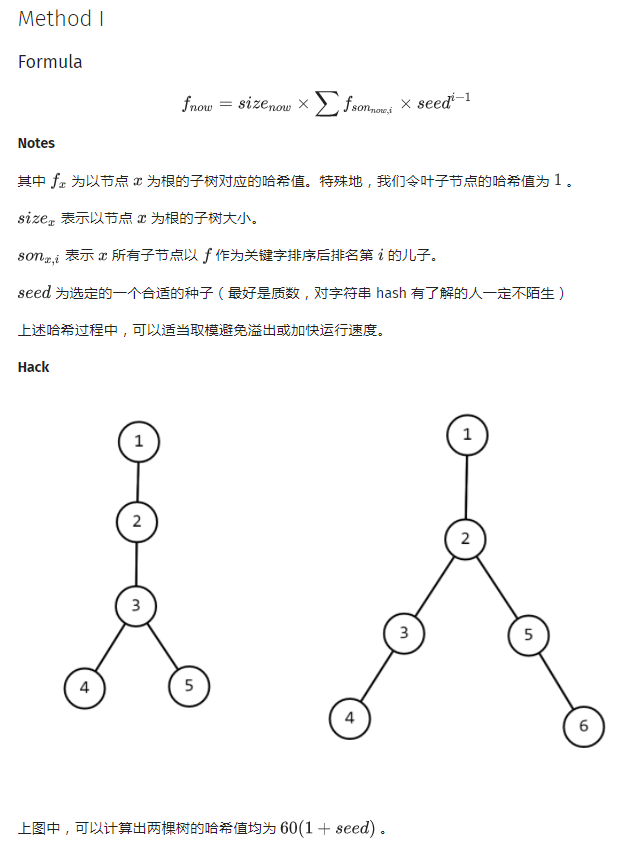
\includegraphics[width=4in]{tree_hash1.png}\\
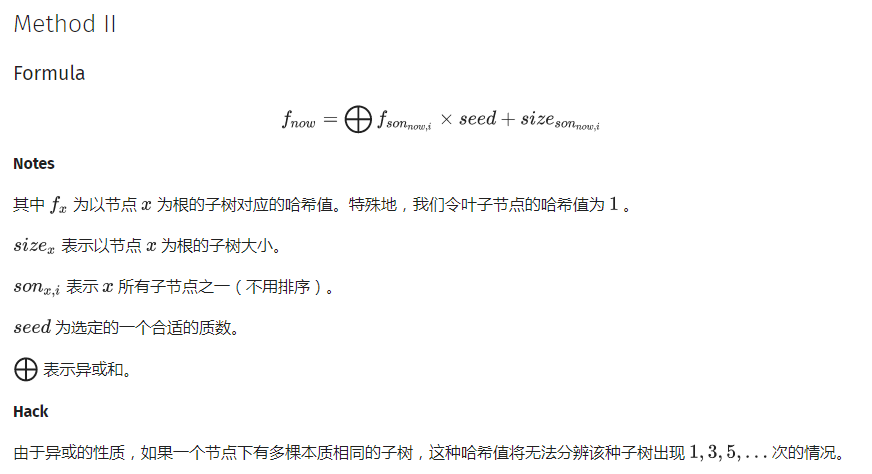
\includegraphics[width=4in]{tree_hash2.png}\\
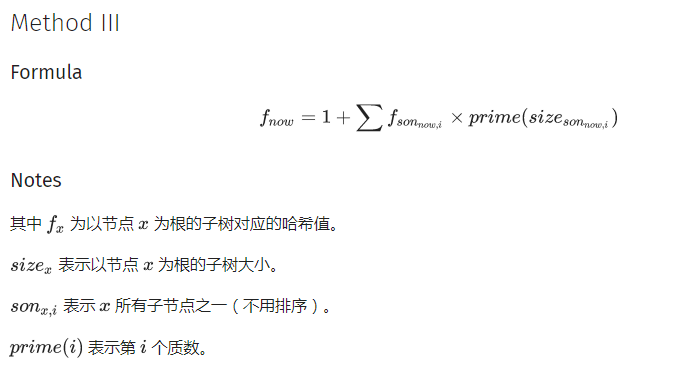
\includegraphics[width=4in]{tree_hash3.png}\\

\end{spacing}
\subsection{线性基求交}
\lstinputlisting{附录/线性基求交.cpp}
\end{document}